%\documentclass[fontsize=12pt, paper=a4, headinclude, twoside=false, parskip=half+, pagesize=auto, numbers=noenddot, open=right, toc=listof, toc=bibliography]{scrreprt}
\documentclass[12pt, conference]{IEEEtran}
% \documentclass[10pt,a4paper]{report}
\usepackage[utf8]{inputenc}
\usepackage[english]{babel}
\usepackage[automark]{scrpage2} % Kopf- und Fußzeilen
\usepackage{graphicx}
\ifCLASSOPTIONcompsoc
    \usepackage[caption=false, font=normalsize, labelfont=sf, textfont=sf]{subfig}
\else
\usepackage[caption=false, font=footnotesize]{subfig}
\usepackage{amsmath}
\usepackage{amsfonts}
% \usepackage{pagestyle}
\usepackage{amssymb}
\usepackage[left=2cm,right=2cm,top=2cm,bottom=2cm]{geometry}

% start new chapters on same page
\usepackage{etoolbox}
\makeatletter
\patchcmd{\chapter}{\if@openright\cleardoublepage\else\clearpage\fi}{}{}{}
\makeatother


\begin{document}
\pagestyle{empty}
\onecolumn

\clearscrheadings\clearscrplain
\begin{center}
David Steiman, 338864 \\

\vspace{8cm}

\begin{Huge}
Design, Development, and Evaluation of a blockchain-based Decentralized Access Control Protocol for Microservices \\
%Building decentralized access control list for microservices on the Ethereum blockchain.
\end{Huge}
\begin{Large}
Bachelor thesis expose \\
\end{Large}
Version 5 \\


\end{center}
\clearpage

\twocolumn
\pagestyle{useheadings}

\tableofcontents

\section{Context}
In a microservice / federated architecture, there are different demands on security. The focus of today's microservice sources is mostly for authentication (e.g. OpenID, IAM, SAML) and authorization (e.g. OAuth 2, JWT). For more fine-grained security, there are different models of access control enforcement, like role based access control (RBAC) or attribute based access control (ABAC). These concepts are simple, but lack on expressibility in complex access control requirements.  For fine-grained access control, ACLs are used for a detailed definition of policies. As ACLs are more complex, they need to be persisted in a way accessible to all microservices. Someone also has to manage the concrete ACL configuration. In particular in federated systems, where services belong to a certain party, every member has to trust this policy administrator.
Consequently the basic idea of ACLs, which often occur in monolithic applications, lacks in two points: decentralization and trust.

I am relying on the model of domain-based distributed systems, which generally describes a domain as ``the realm of knowledge or the activity that is of interest to the users of the software system being designed`` \cite{b2} and which ``can be used to group
objects in a hierarchical structure, to apply a common security policy, to reflect
organizational or geographical structure, or to partition the security management in order
to cope with the complexity of large distributed systems.`` \cite{b1} Based on the concept of Yialelis, which is close to a system this thesis aims for, access control can be expressed in ``access control lists`` (ACL), which contains the requesting subject, requested target and access rules defined for those. Policies are enforced by a reference monitor. But his concept assumes the presence of a policy administrator, which is performing the overall security configuration. So this access control mechanism requires trust in a central authority. \\

One way to remove the need in trust is moving the coordination of any state changes of the current policies to a smart contract, which runs on a blockchain. In particular, Ethereum offers a advanced blockchain, where code instructions are treated as transaction, which run on an large computation network. Once deployed, neither the state nor the instructions of this code can be changed, so there is no need to trust a third party with global privileges.

Anyway, none of the sources deals with the persistence of the stored policies. According to microservices, storing such information should not depend on a single storage.

So the idea of this thesis is to design an access control mechanism, which is fully decentralized and trustful. In details, that means no single member is responsible of managing or storing the policies.

% One of the today's distributed trust pioneers is blockchain technology, which generally enables trustlessness to any kind of transactions. In particular, Ethereum offers a blockchain, where smart contracts can be executed. The result is a decentralized application platform, which executes code trustfully. This, for instance, allows building tamper-free voting systems.

\begin{figure}[!h]
  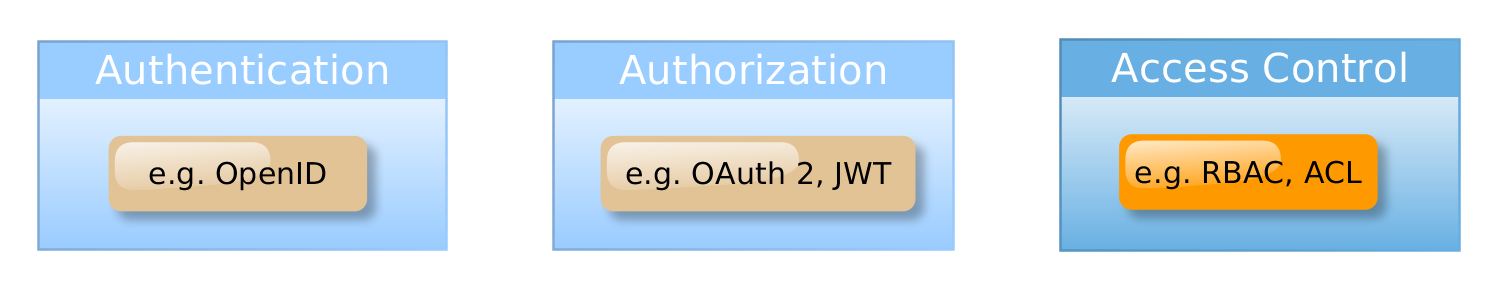
\includegraphics[width=\linewidth]{figures/access-control.png}
  \caption{DACL for access control in microservices.}
  \label{fig:access-control}
\end{figure}

The idea of this thesis is to design and develop an access control mechanism called DACL (decentralized access control list), which stores its state in IPFS and coordinates changes to the policies by voting on proposals using Ethereum smart contracts. Both parts implement a 2-protocol-system defining an access decision and a policy coordination protocol. This mechanism assumes that authentication and identity management already exist, so it is possible to determine at request time the requesting subject, the target and the operation to match it with the ACL entries. After matching, policy enforcement is done using the access decision protocol. The second protocol is being used to trustfully read the policies and coordinate changes on the ACL. Instead of requiring a policy administrator, changes to the policies can be proposed by any participant (e.g. a microservice, a platform owner etc.). All participant place votes on these proposals by using the policy coordination protocol and let the smart contract take the final decision for the changes to be committed. During the thesis, the mechanism will be applied to an exemplary scenario to show, how these protocols should be used and implemented.



\section{Example scenario}

\begin{figure}[!h]
\centering
  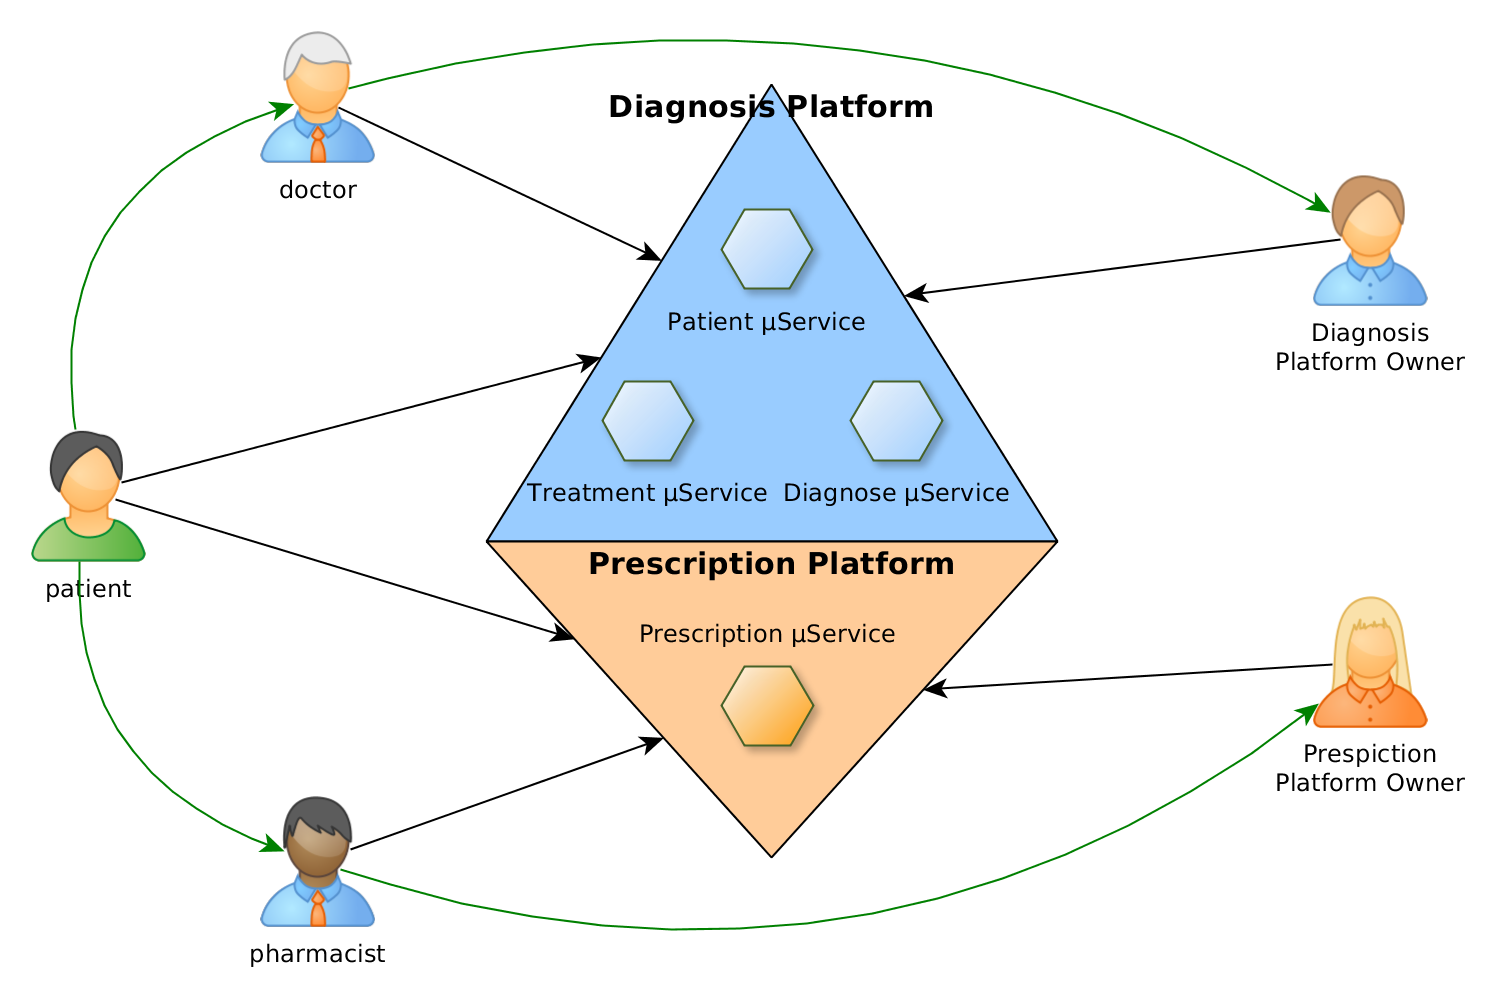
\includegraphics[width=\linewidth]{figures/platform.png}
  \caption{Federated Conference Platform.}
  \label{fig:platform}
\end{figure}

The scenario describes a federated application platform for papers, reviews, and ratings. Authors can upload papers, which are reviewed by reviewers. Accepted papers are then open to be rated by users of the rating platform. These processes can be done on the platform in figure 2.1. It is realized with microservices, which provide endpoints for their domain objects. The figure shows two parties: papers and rating platform owner. The key question is how to manage permissions, without giving a certain party full access, and protect the data of all participants.

\section{Problems}

\subsection{Specification and precision}
All microservices should operate according to a common mechanism, so new policies can be enforced in a uniform way.

So at first, there should be a protocol, which defines how the ACL looks like and how a participant should interpret it. As talking about domain object security, the proposed solution should be able to define fine-grained security setting. This means it must deal with common terms like subjects/principals, targets, and permissions.

\subsection{Blockchain design}
There are several problems specific to Ethereums smart contract system and the blockchain itself. Every writing operation costs some fees in ether to be paid by a participant. So this costs must be regulated by the contract with methods like auto-refilling.
%In particular, it needs to be discussed if the public blockchain should be used, forcing all participant to spend money for changing the policies. In contrast: relying on a private test network would remove any costs but also enable majority attacks of a certain participant. 
The DACL smart contract allows a set of participants to be part of a network, where every member is permitted to read the ACL, make proposals and place votes. As there is no network administrator, the protocol must define how new members can join or how to remove malicious participants.
% More on this, it must be discussed, how the smart contracts should be described. In particular, how privileges to the contract owner are designed in terms of the overall trust.

Another issue is: putting data on the blockchain is expensive, so it must be clarified, which data is stored ``on-chain`` and which ``off-chain``. In particular, what kind of tool should be used for storing off-chain?

The basic idea says every participant can read, propose and vote. This leads to a proposal being forced to be voted by all participants. But there are use-cases, where it is needed to maintain participant which do not vote for some reasons. 

\subsection{Consensus finding}
Another point is how to reach consensus in the network. If multiple policy change proposals are pending and the network must end up in a consistent state, where all valid policy change proposals are checked in. 

One idea would be to force every party to provide changes by offering a complete state of the previous ACL including the changes, so other parties must check the entire ACL in order to accept it. This keeps the ACL collision free and during finding consensus, all participants are referring to a state, which was accepted by the entire crowd earlier. As an alternative, one participant may provide a delta to the current state, which claims to be a valid successor of the last accepted delta. Accumulating all deltas will give the current state. Here, only the new changes must be voted on by the participants. Merging is simpler than voting on complete states, but it is possible that valid forks with internal contradictions might happen.

\subsection{After-the-fact changes}
When data is stored on the blockchain, there still are business use-cases to make exceptions on facts. To cover those exceptions the Hyperledger requirements work group released a set of 8 requirements \footnote{Deventer, Joosten, 2017}, where the following are relevant to the DACL design:

\begin{itemize}
\item{a member(anchor) shall be able to sign over its authorization to another member (guardian) after the fact. This requirement accords to the following two scenarios:

\item{anchor loses its authorization}
\item{anchor maintains its authorization over the smart contract}
}
\item the network shall be able (e.g. via a blockchain consortium) to sign over the authorization over a smart contract from anchor to another member
\item it should be possible to re-assign the authorization
\item all assignments shall not require handling over private keys
\end{itemize}

As the DACL doesn't define a consortium, the other requirements don't fit well here.



%Using blockchain technologies provide the safeness, that once information is stored in the blockchain, it cannot be changed (if a smart contract doesn't make exceptions on that). But there are still business use-cases when there is need of changing persisted data. There is a list of requirements from the Hyperledger requirements WG, describing several properties a distributed system should comply, in order to allow exceptions on these use-cases.

\subsection{Horizontal scalability of the microservices}
In terms of scalability, DACL should have a minimal impact on the overall horizontal scalability. In particular, if DACL forces a microservice to replicate the huge amount of security states during replicating the services themselves, it could affect the boot-up time or cause latency, because it takes too much time for making access decisions. A vivid example would be if every microservice must first synchronize with the entire Ethereum blockchain from scratch, what would take hours for a new replica to be running.

\section{Proposed solution approach}


\begin{figure}[!h]
    \centering
  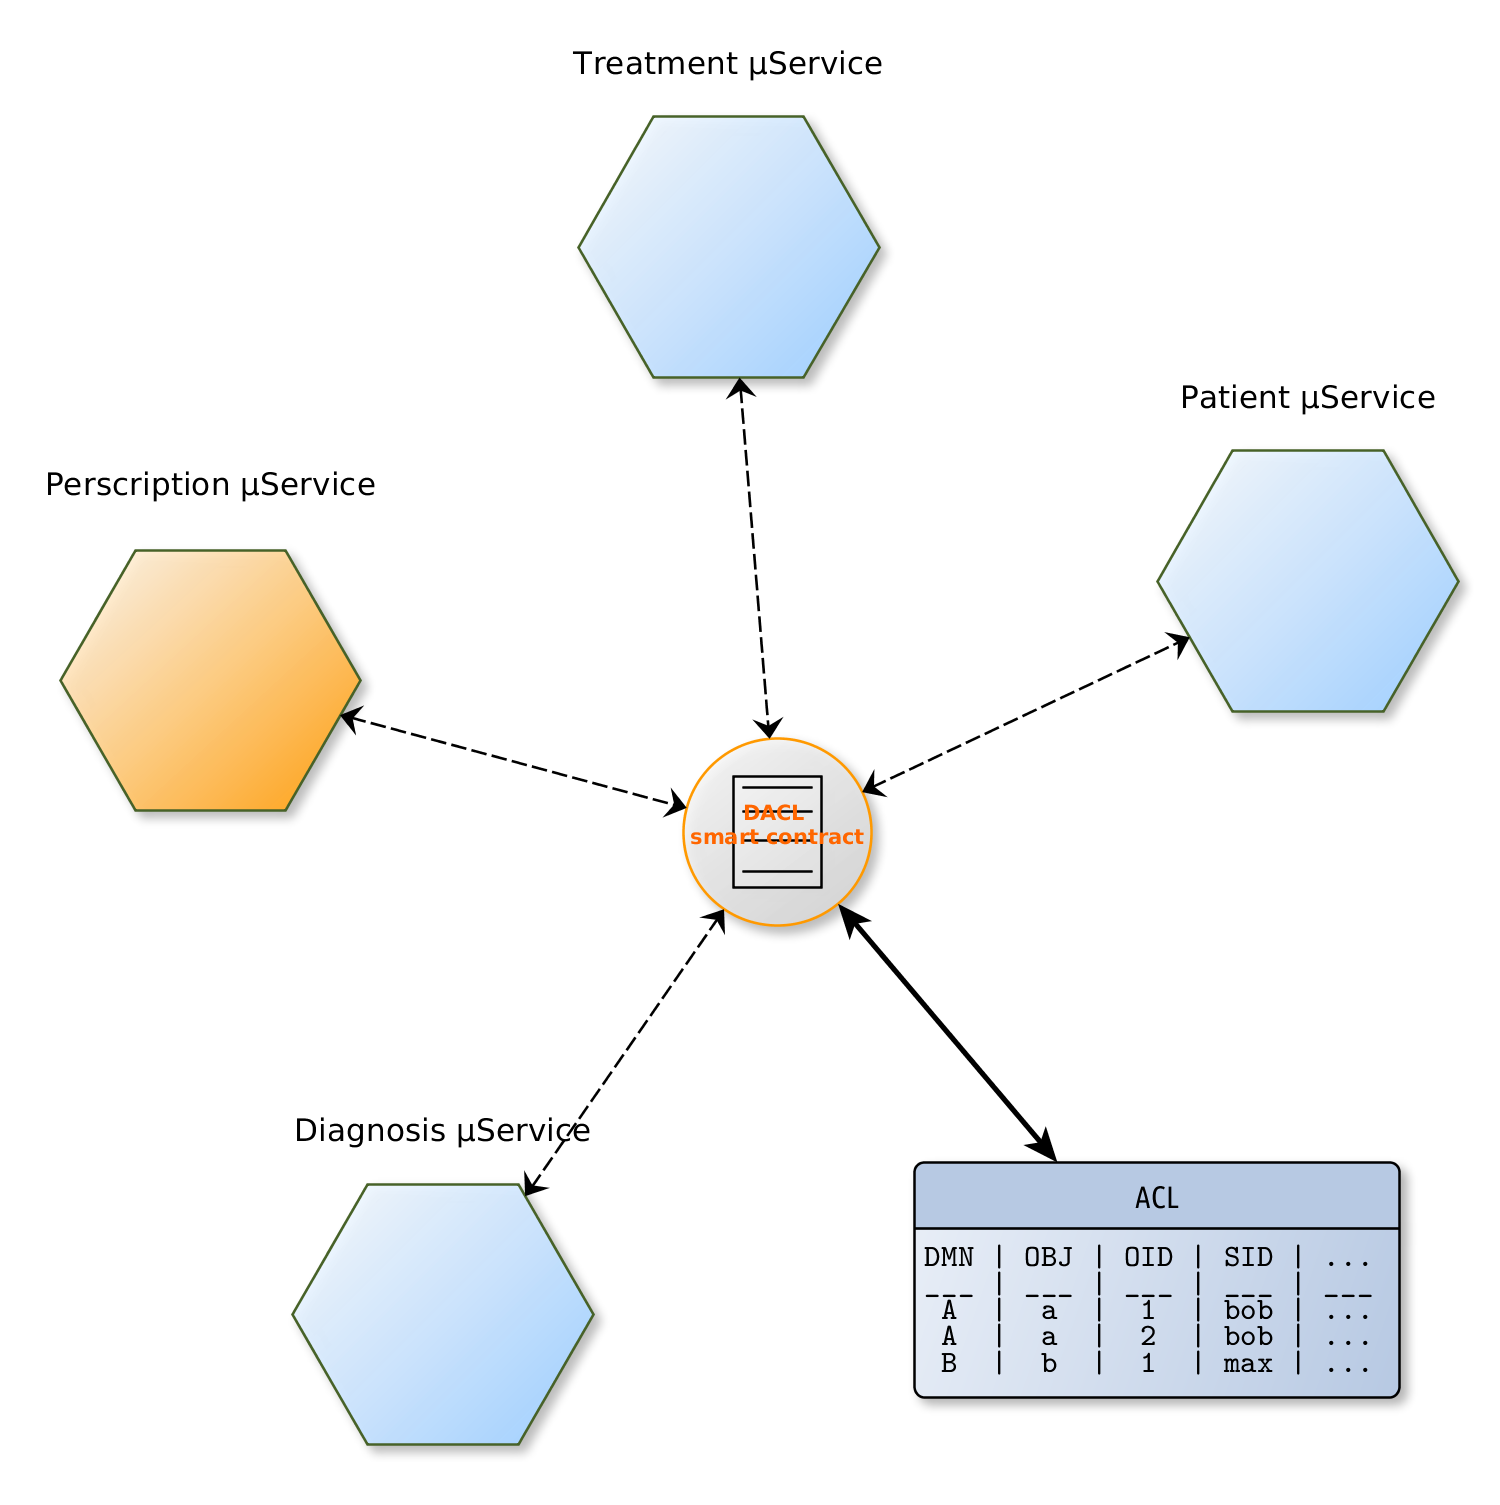
\includegraphics[width=\linewidth]{figures/DACL-basic.png}
  \caption{Basic DACL architecture.}
  \label{fig:basic-dacl}
\end{figure}

The proposed distributed access control list protocol (DACL) claims to give a solution to the problems. At the core, all members of the DACL defined network interact with a single smart contract, which provides the actual state of the ACL and coordinates changes on this state. 

\newpage

\subsection{the DACL protocols}

DACL is designed using the following sub-protocols:

\subsubsection{access decision protocol}

The protocol first defines an access control entity $ ace \in \mathbb{ACL} $, which is in an access control list $ \mathbb{ACL} $, defined by:
\begin{footnotesize}
$
\mathbb{ACL} = \{ (domain, oid, uid, sid, permission, order) : domain, oid, uid, sid \in \Sigma^*,  permission \in \{0,1\}^4, order \in \mathbb{N} \} 
 $
 with: \\
 $ domain = $ the domain that owns the object  \\
 $ oid = $ the object identifier of target object \\
 $ uid = $ the objects unique identifier \\
 $ sid = $ the unique identifier of the requesting subject \\
 $ permission = $ 4 bits for create, read, update and delete permission \\
 $ order = $ the order of this entry in a set of matched rows \\
 \\
\end{footnotesize}
This infinite discrete set can be represented as the following table:

\begin{table}[!h]
\begin{tabular}{|c|c|c|c|c|c|}
\hline \rule[-2ex]{0pt}{5.5ex} domain & OID & UID & SID & permission & order \\ 
\hline
papers & paper & 123 & Alan & 0-1-1-1 & 1 \\ 
papers & paper & 123 & @any & 0-1-0-0 & 2 \\ 
papers & paper & @any & @any & 1-0-0-0 & 3 \\ 
\hline
\end{tabular}

\end{table}


Every microservice acts as a participant for a domain (by owning a private key known to the smart contract). 

To evaluate this ACL for a given object and subject, a participant iterates over all access control entries for its matching domain in the defined order. The first match is providing the decision if access is granted. A participant, is free to use any convention for identifying a single principal, a group of users or a role. 


\subsubsection{policy coordination protocol}

The policy coordination protocol describes how exactly parties can change the ACL. Given the fact, all communication is done via the DACL smart contract, the following figure describes how a successful reconciliation should proceed 

\begin{figure}[!h]
\centering
\subfloat[initial state]{
	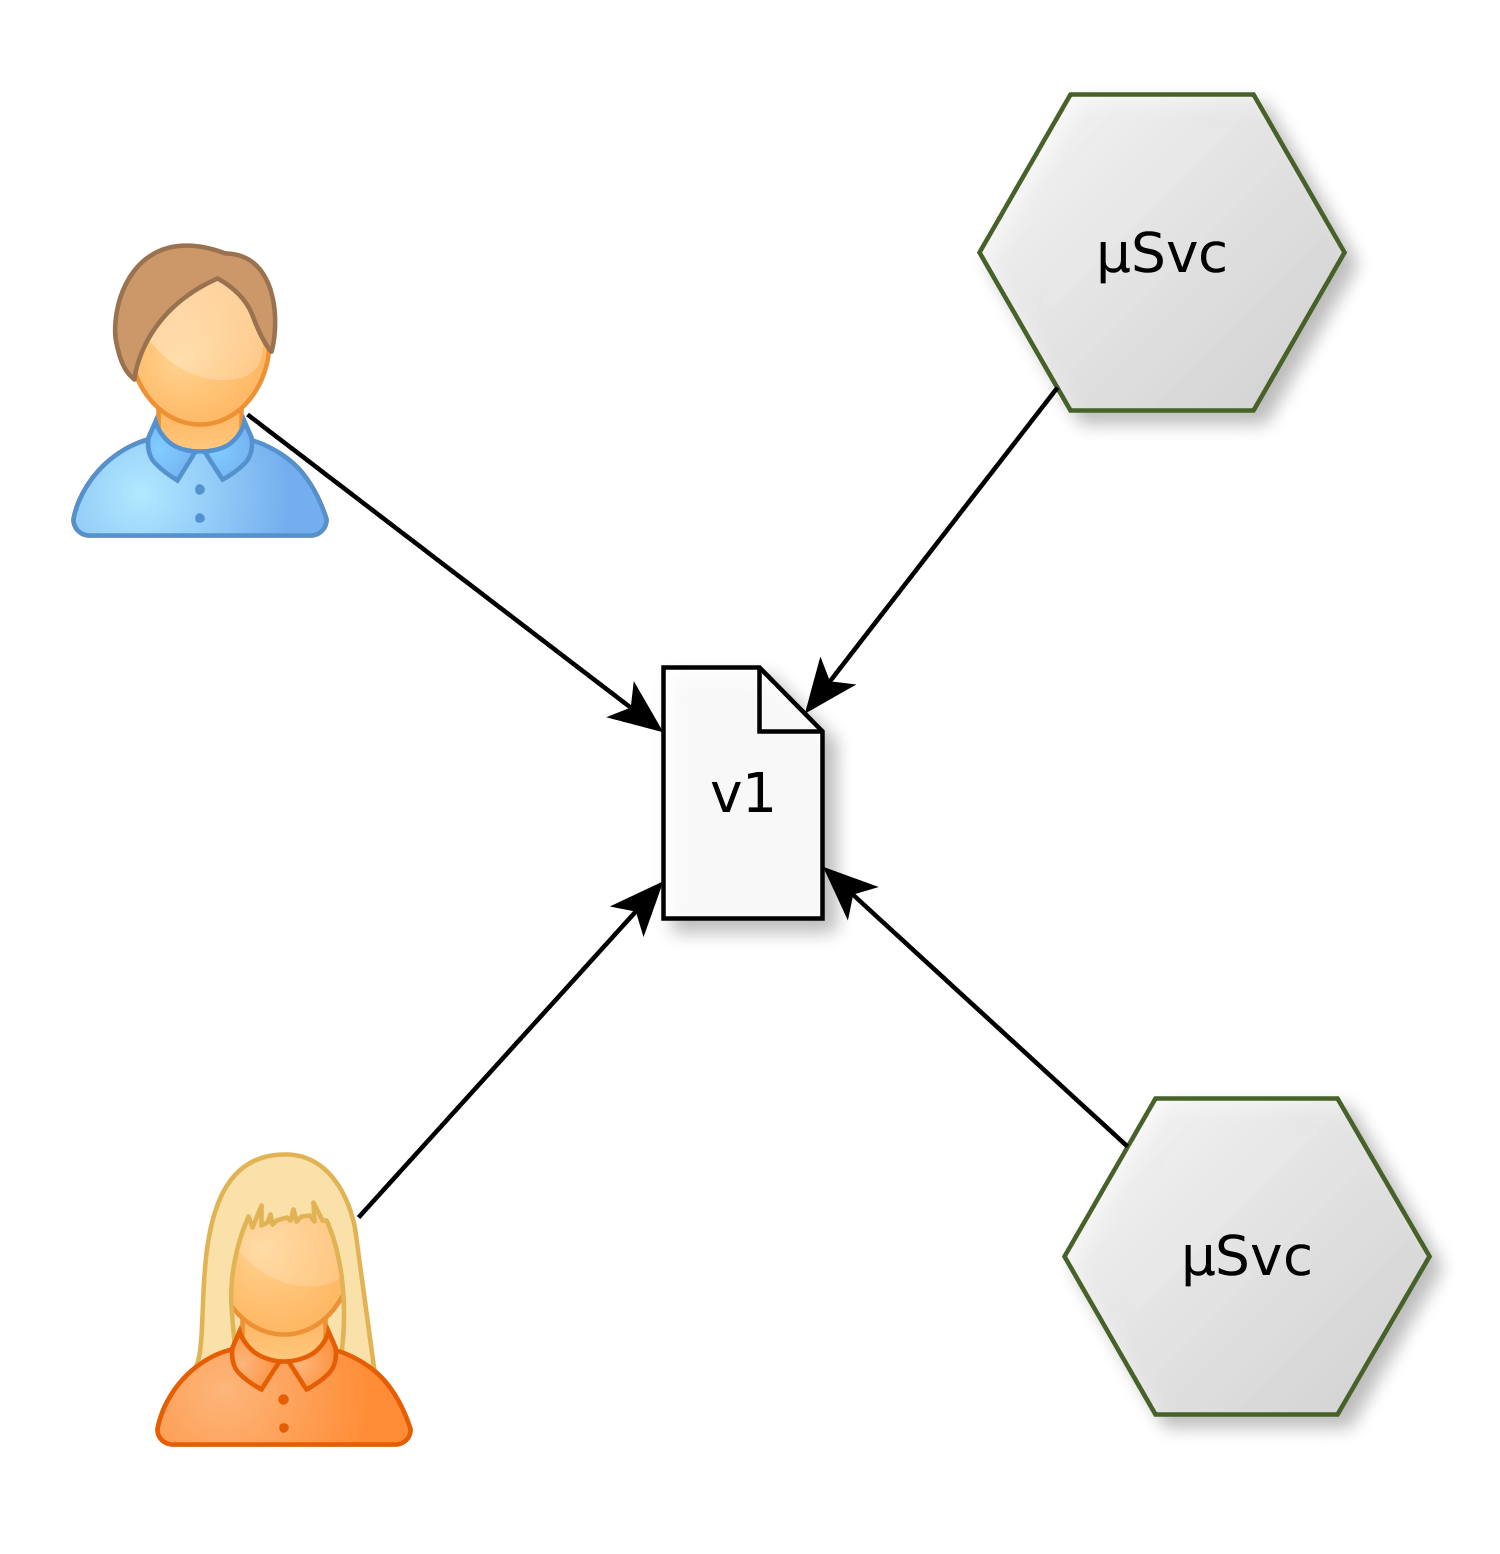
\includegraphics[width=0.32\linewidth]{figures/ACP-initial.png}
} \hfill
\subfloat[state change proposal]{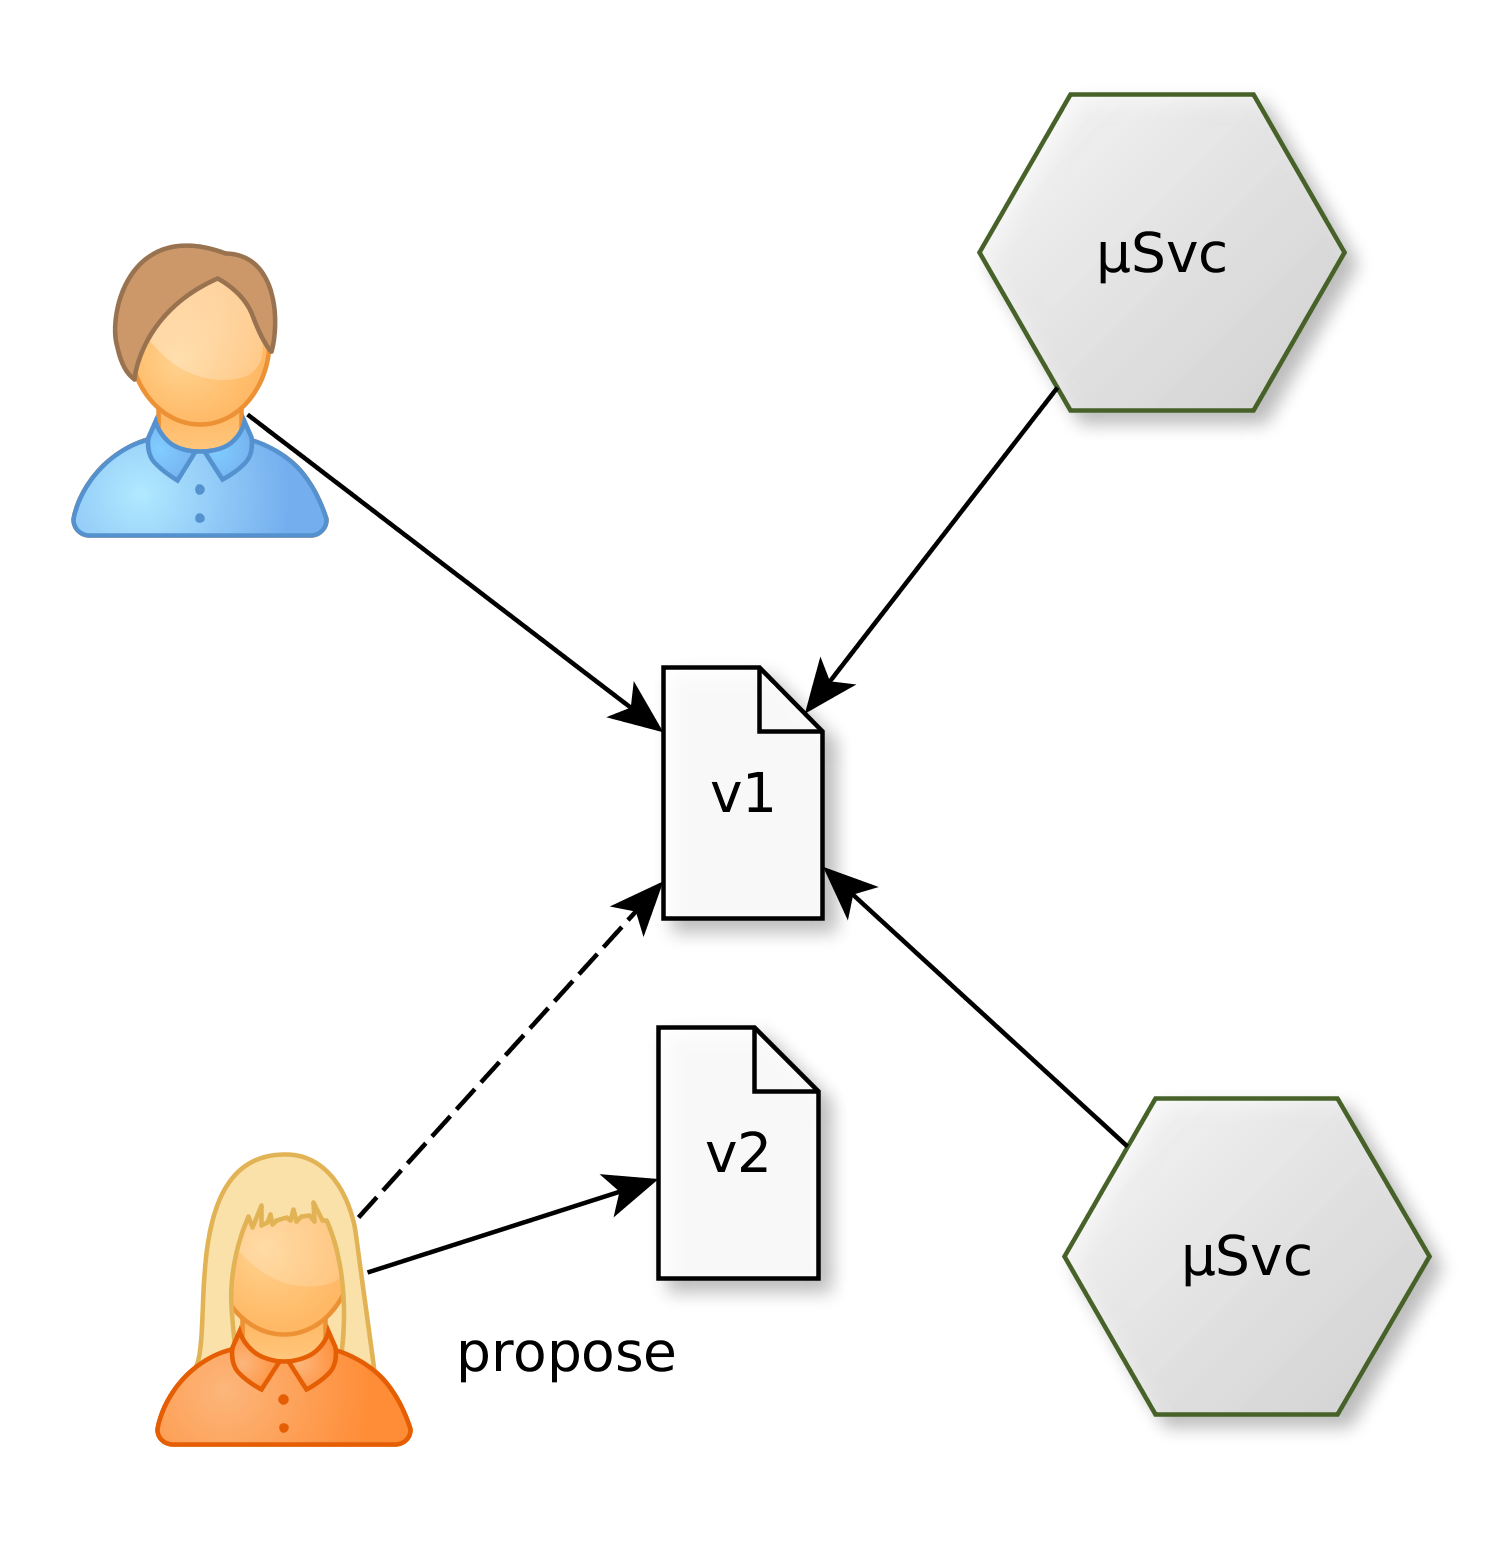
\includegraphics[width=0.32\linewidth]{figures/ACL-propose}} \hfill
\subfloat[accepting new policy]{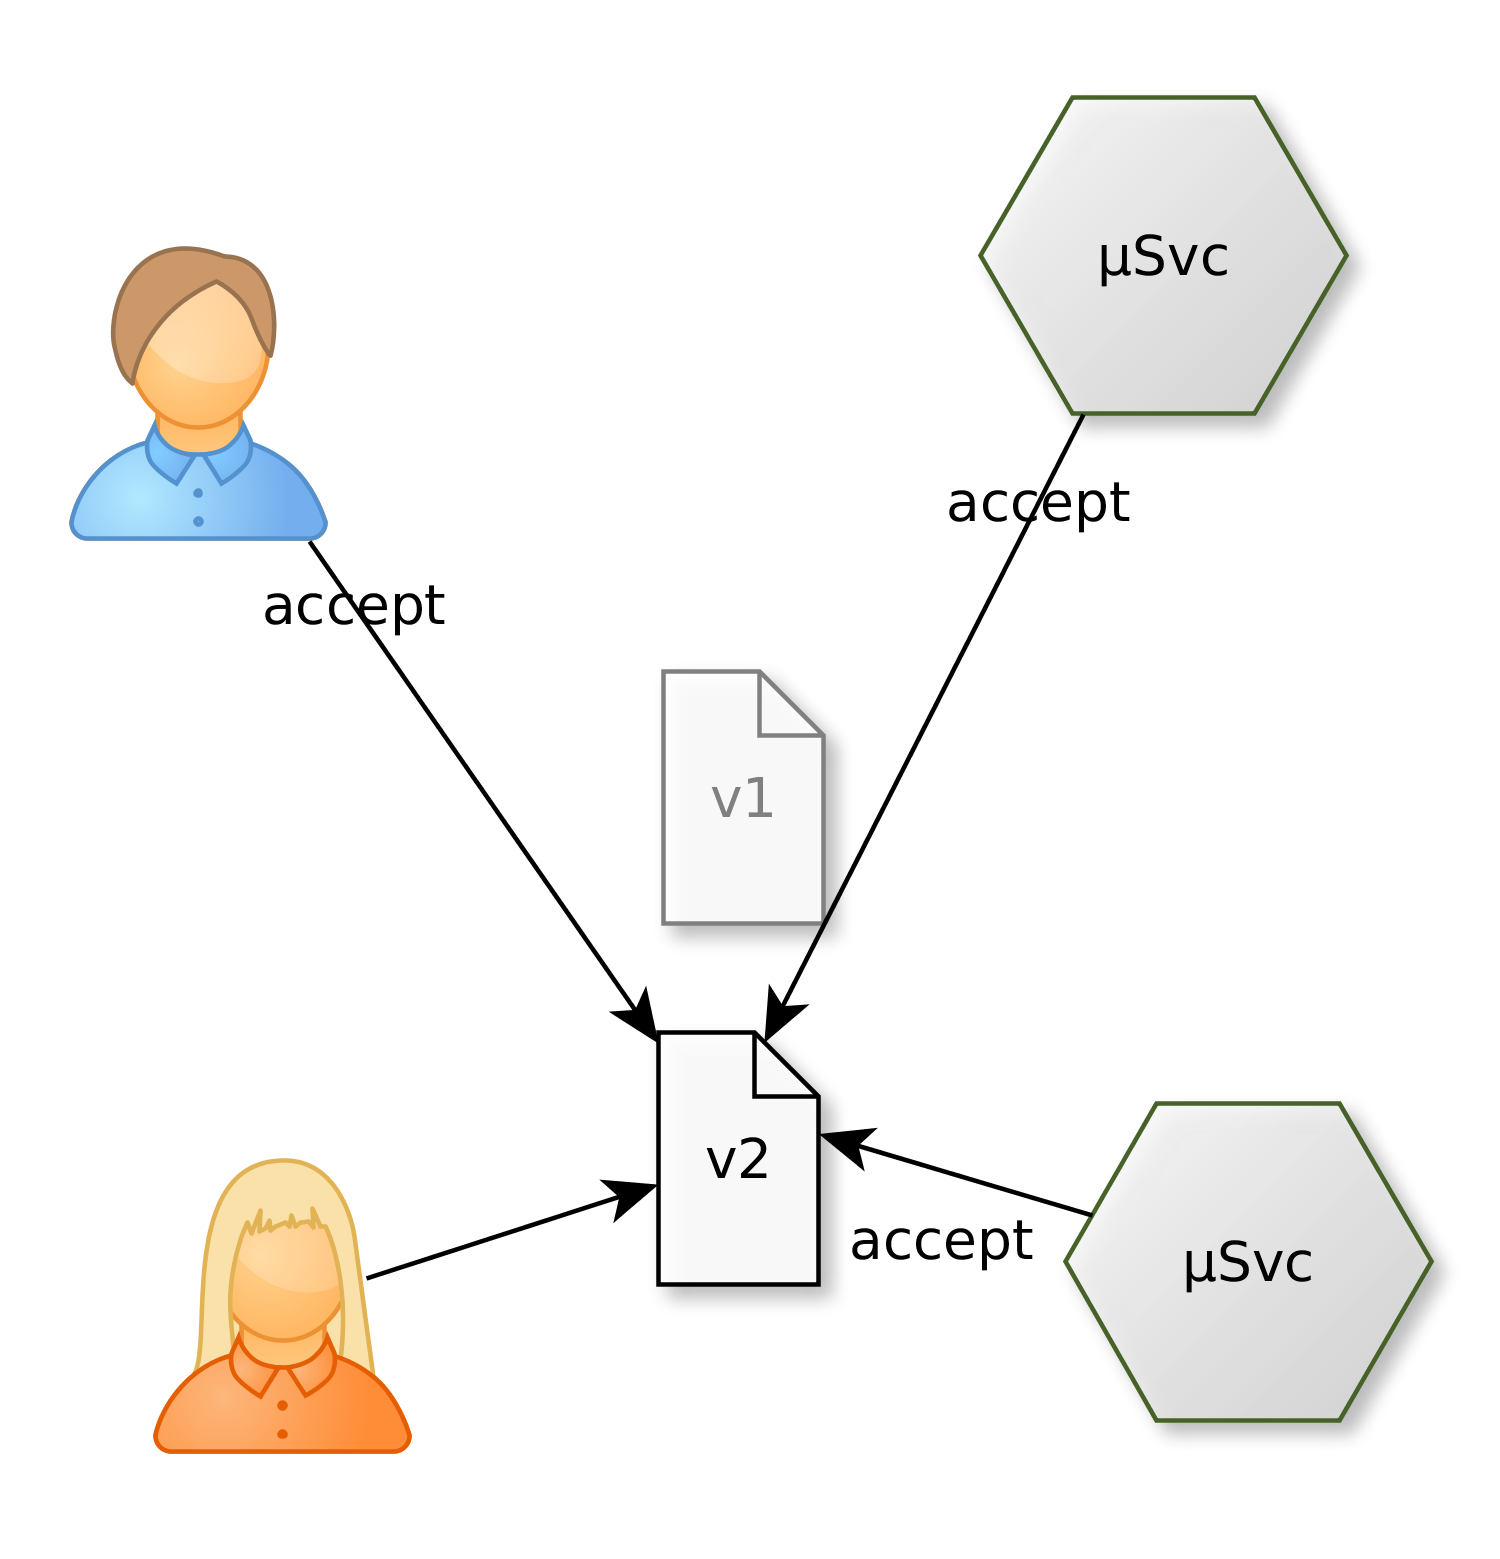
\includegraphics[width=0.32\linewidth]{figures/ACP-accept.png}} \\
\caption{test}
\end{figure}

%\begin{figure}[!h]
%\minipage{0.32\textwidth}
%
%  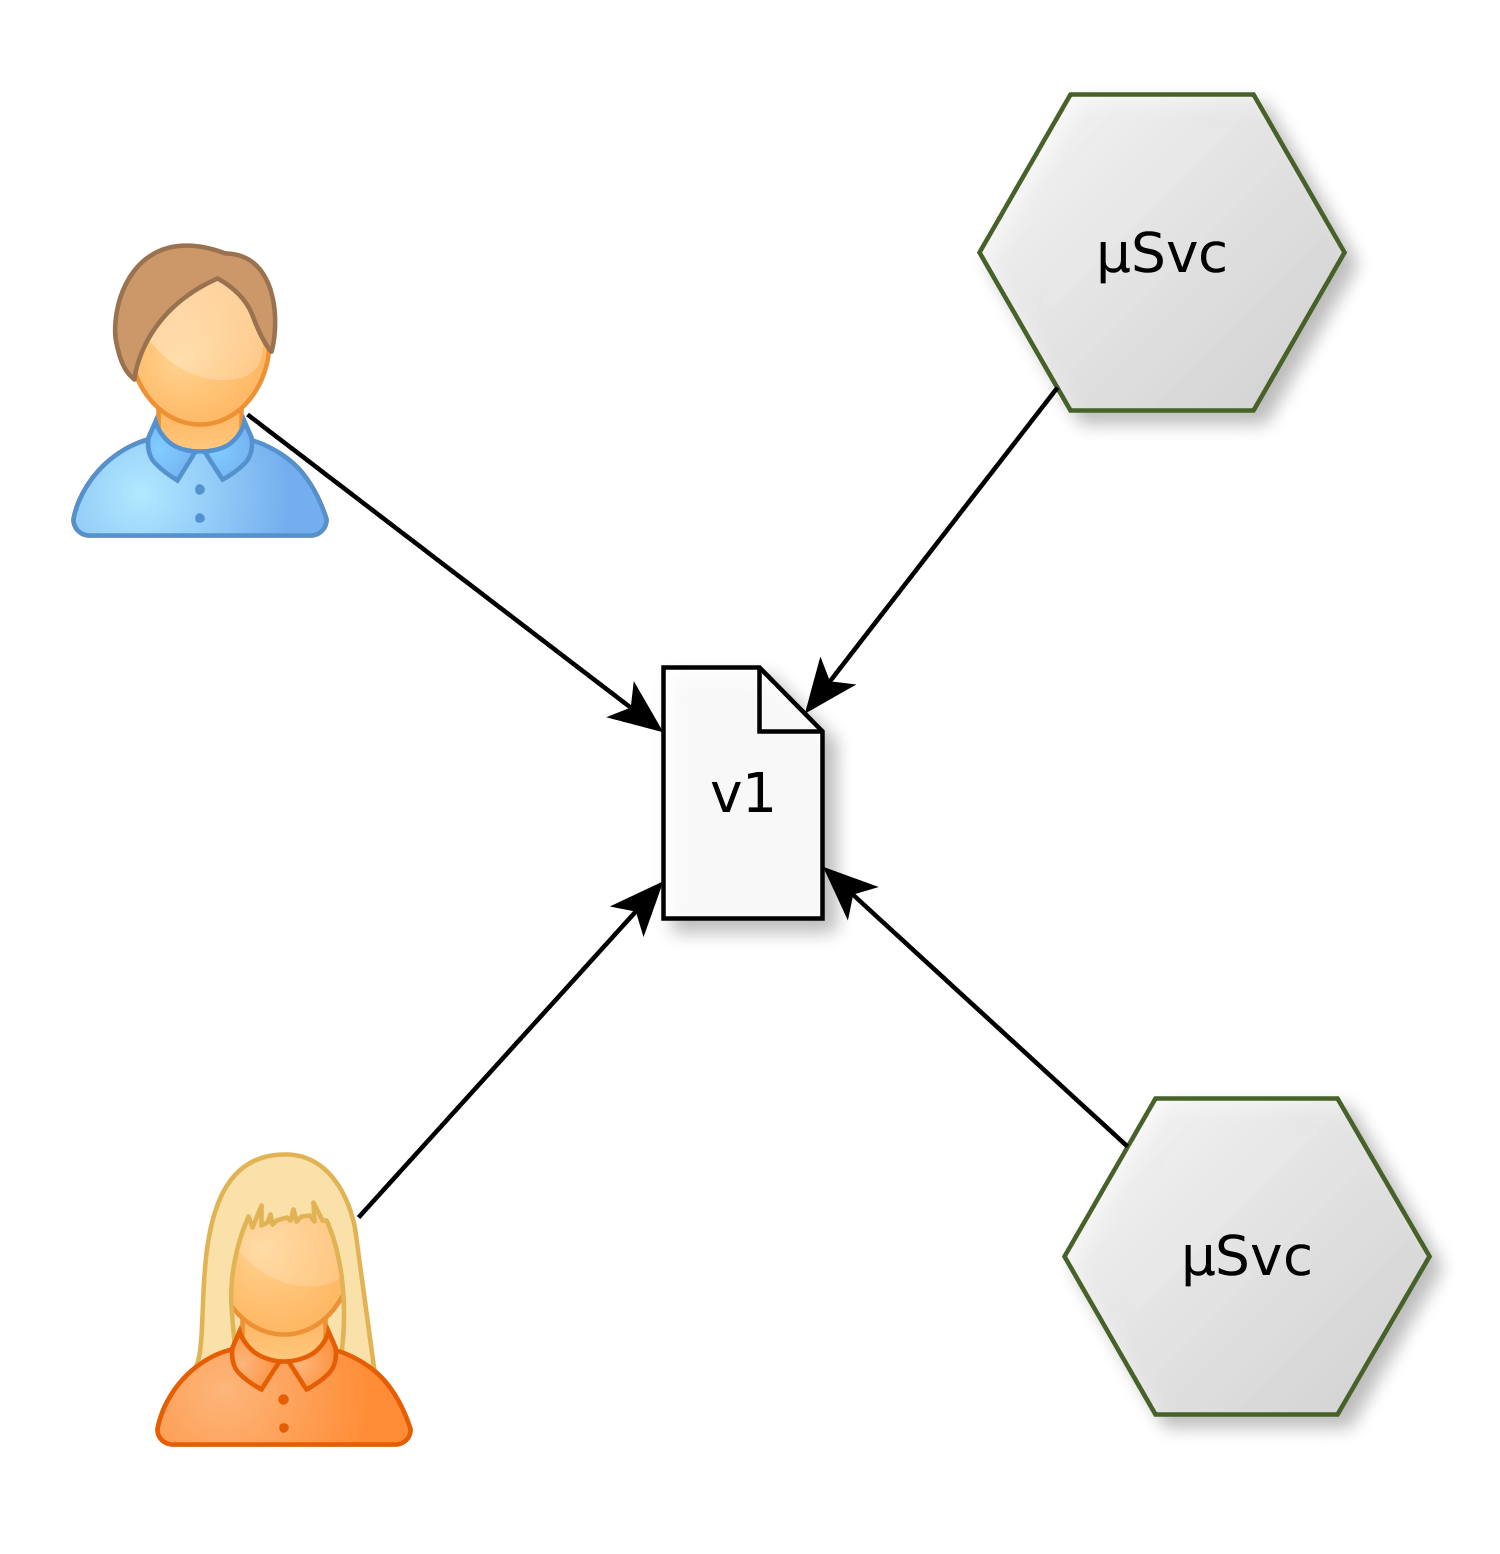
\includegraphics[width=\linewidth]{figures/ACP-initial.png}
%  \caption{initial state}
%  \label{fig:acp-init}
%\endminipage\hfill
%\minipage{0.32\textwidth}
%
%  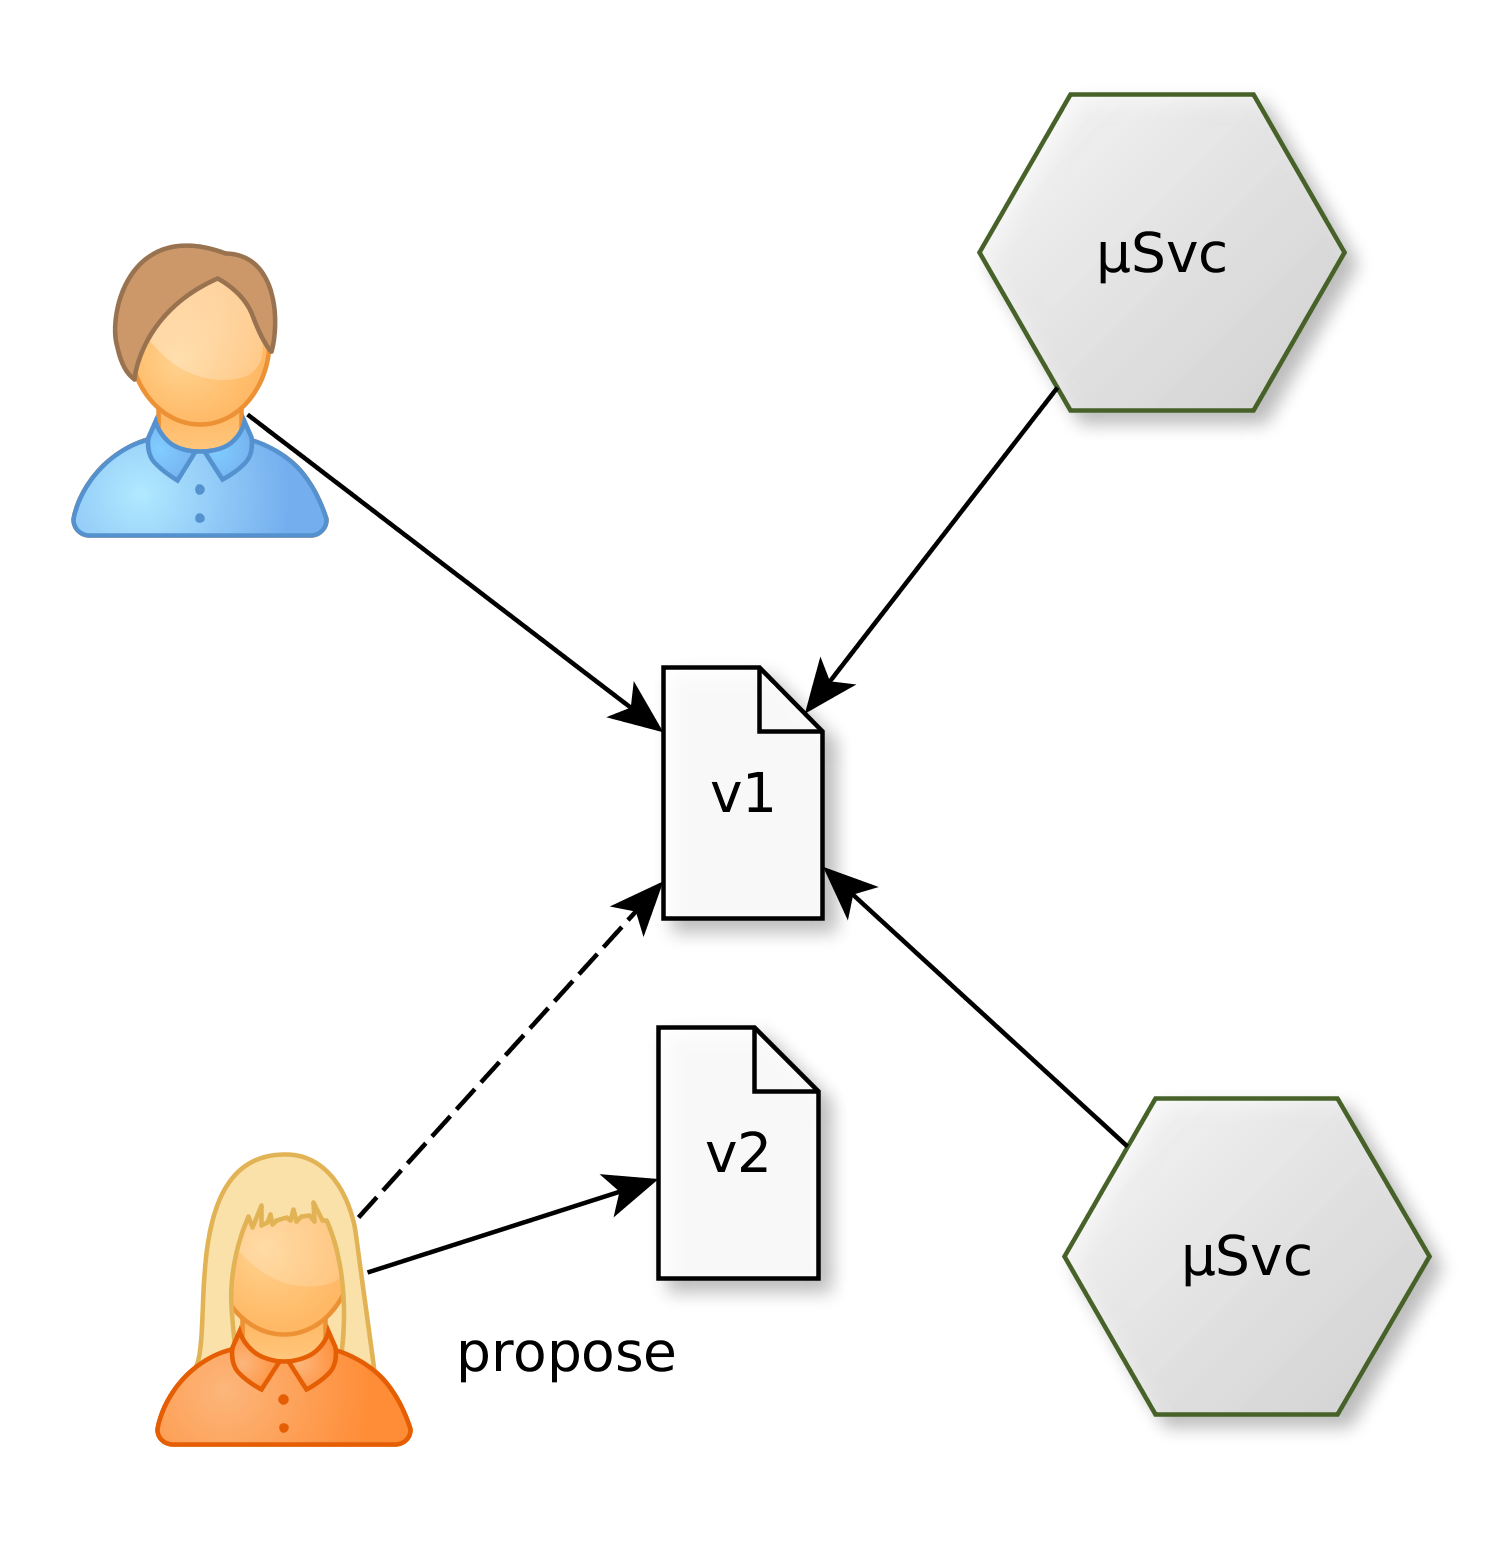
\includegraphics[width=\linewidth]{figures/ACL-propose.png}
%  \caption{state change proposal}
%  \label{fig:acp-propse}
%\endminipage\hfill
%\minipage{0.32\textwidth}
%
%  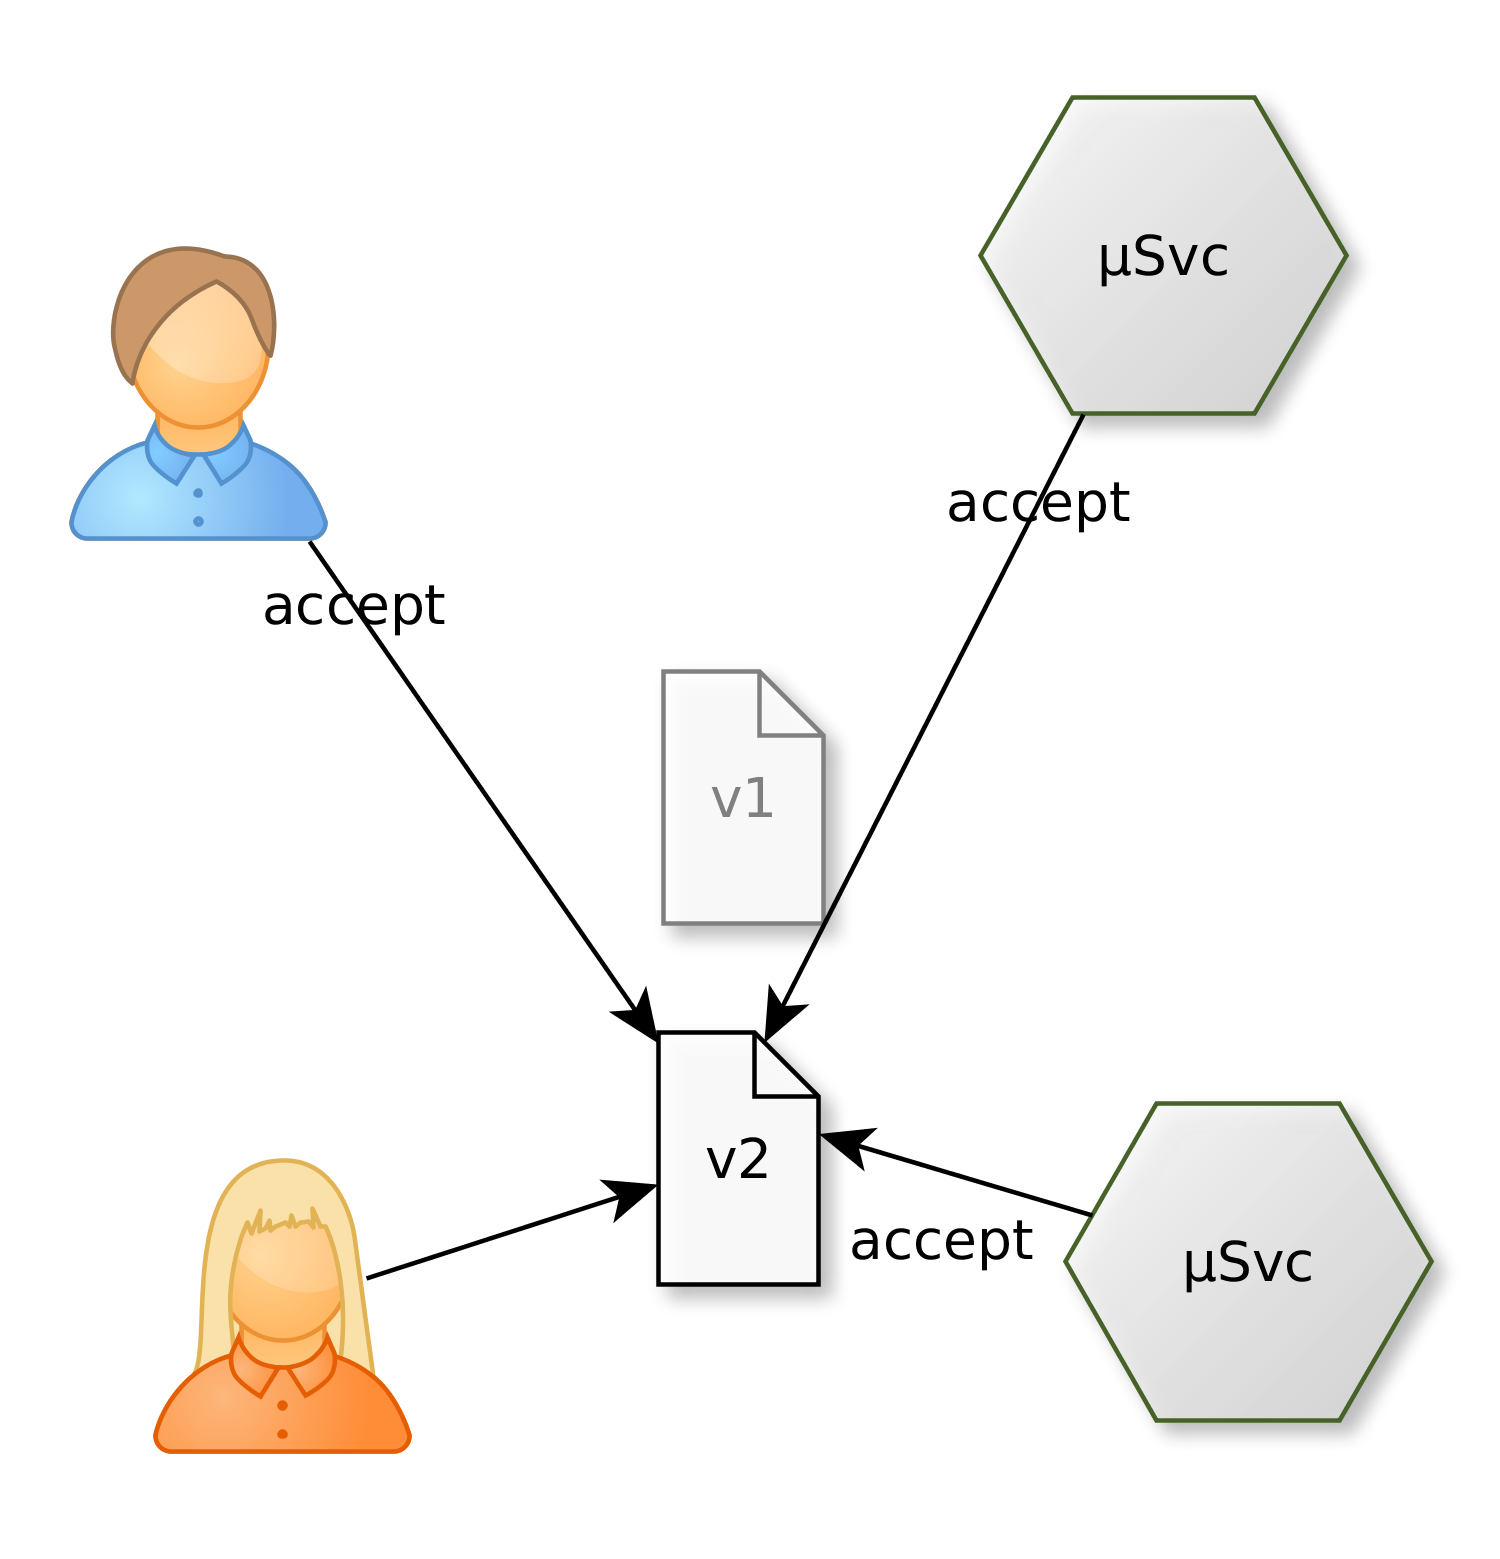
\includegraphics[width=\linewidth]{figures/ACP-accept.png}
%  \caption{accepting new policy}
%  \label{fig:acp-accept}
%\endminipage\hfill
%\end{figure}

When a participant wants to change policy rules, he defines a new version of the ACL and reports a proposal to the network. Each participant can either accept the new version, deny with a user defined reason or abstain from giving an answer. If no of the participants denies the proposal, the smart contract provides the new ACL list. 

As an alternative, participants could send deltas instead of full versions of the ACL.\\


\subsection{implementation and on-chain/off-chain design}

\begin{figure}[!h]
  \centering
  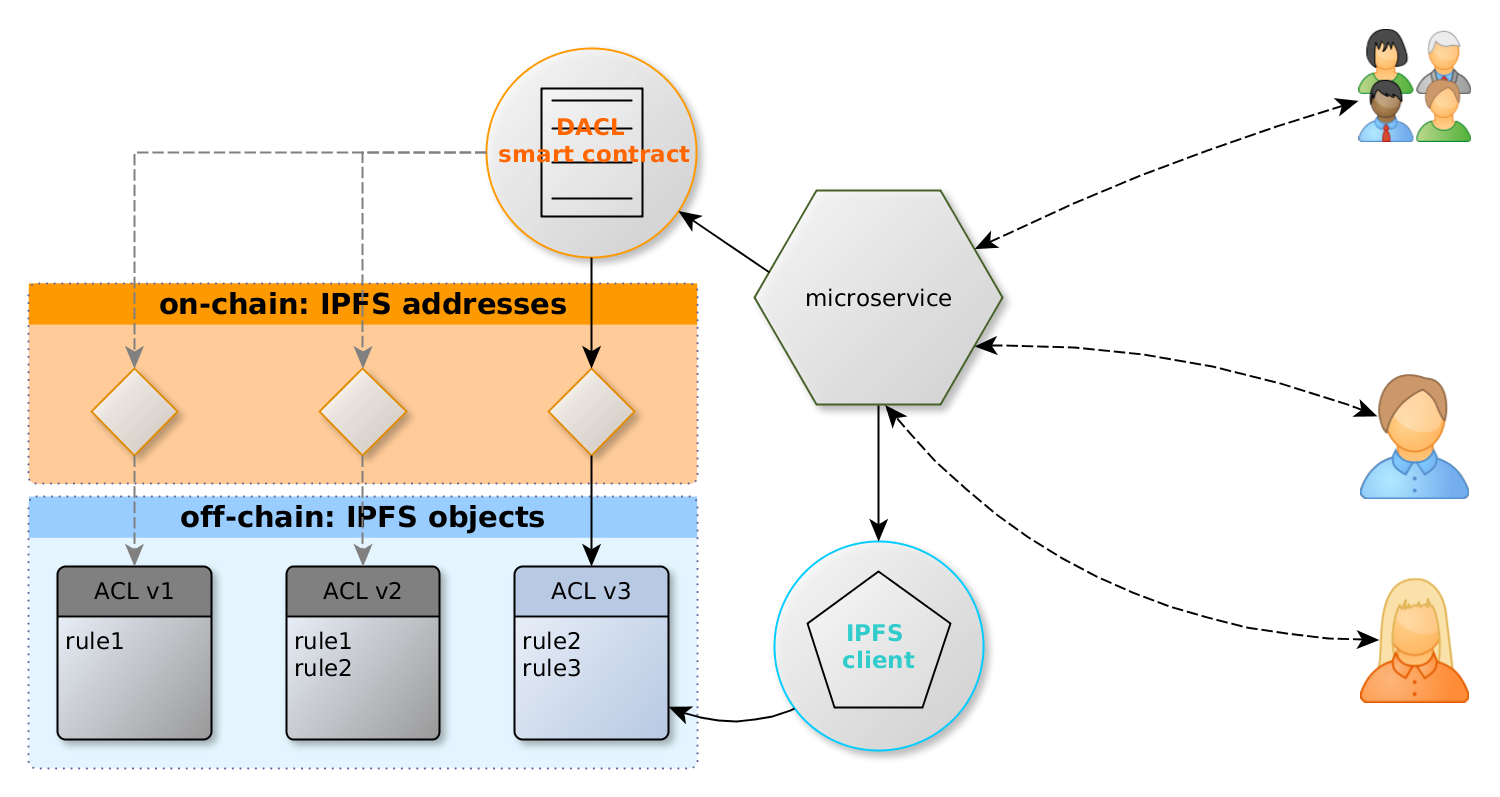
\includegraphics[width=\linewidth]{figures/eth-ipfs-design-without-client.png}
  \caption{DACL architecture}
  \label{fig:ipfs-design-without-client}
  \centering
\end{figure}

After defining that protocol formally, a reference prototype must be implemented using a common language for building microservices. The example will be implemented using NodeJS and Solidity (for developing smart contracts). 

To keep as little as possible data on the blockchain, the smart contract will store IPFS addresses of objects. In the most basic scenario every microservice implements the policy coordination protocol directly when interacting with IPFS and ethereum. 

In order to standardize the coordination, a DACL client can be developed that runs parallel to each microservice and makes the protocol processes available via a well-defined API. It interacts with the smart contract, reads the address from the blockchain and opens the content using an IPFS client.

\newpage

\begin{figure}[!hb]
  \centering
  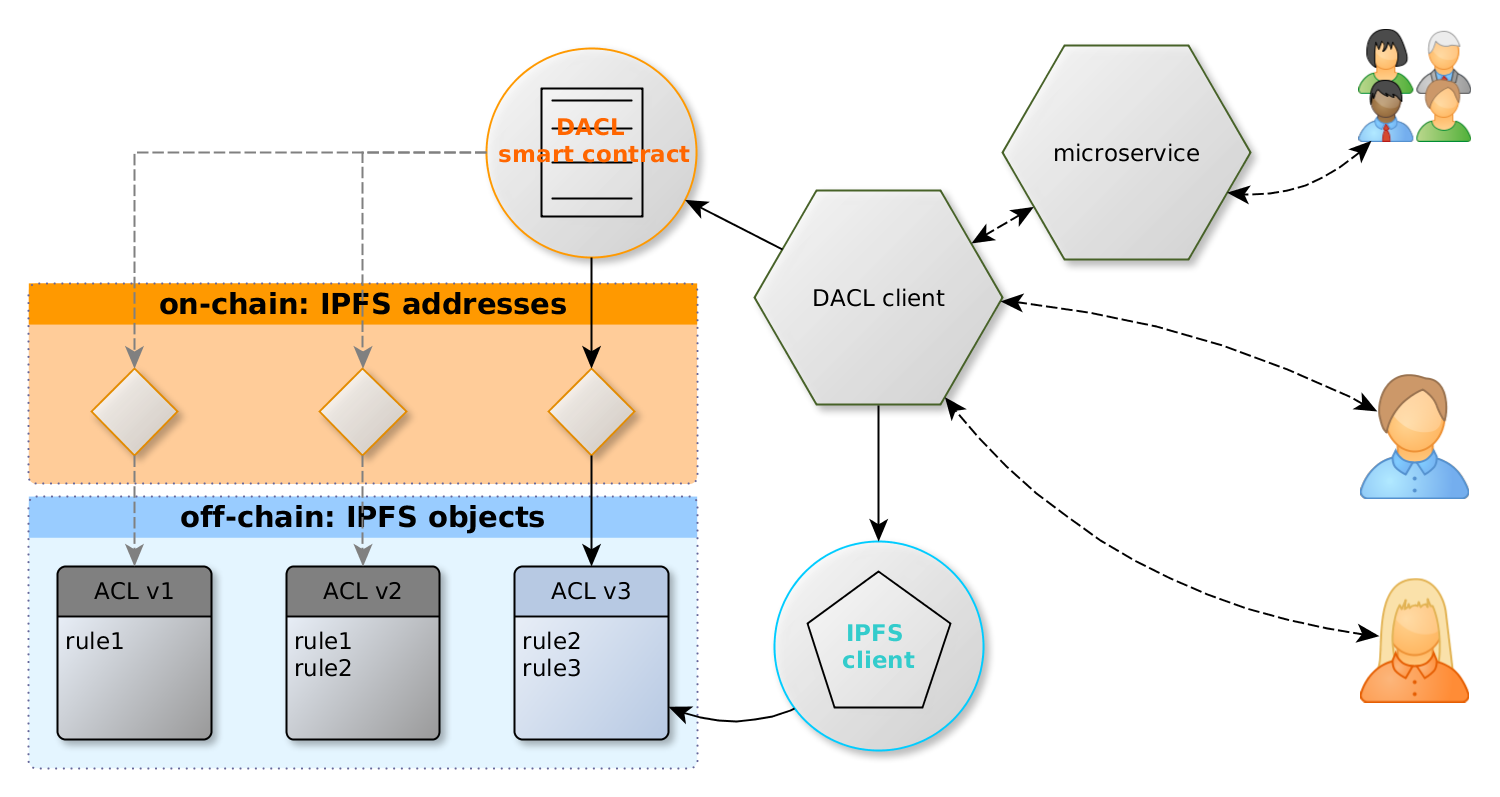
\includegraphics[width=\linewidth]{figures/eth-ipfs-design-with-client.png}
  \caption{DACL architecture with client}
  \label{fig:ipfs-design-with-client}
  \centering
\end{figure}


%
%Each microservice reads and writes a common policy configuration file, which is stored in IPFS and hashed in the Ethereum blockchain. During read, a service must implement own security policies for itself. Interpreting non-owning domain object is optional. For writes (and changes) of that configuration, a service is only able to make a proposal. Using a simple voting system, every service may vote on incoming proposals. Depending on the choice, how consensus is reached, the smart contract finally evaluates pending proposals and in the case of satisfying all conditions, adds the new configuration to the network.



\section{Evaluation}

\subsection{comparing results with problems}

In the first chapters of my thesis, I figure out important properties/objectives DACL claims to satisfy. After implementing the example platform, it can be compared to these objectives. For example the after-the-fact change, where there is a set of requirements to check.

\subsection{attack vectors}

The prototype will consist of various design decisions. Like the question, how to act in a situation, where no clear policy is present (e.g. for e newly created entity and a still pending policy). Furthermore a single participant might block any further changes to the ACL by always denying any new proposals. As there is a currency circulating, which acts as fuel for the systems, it should be checked what happens, when DACL run out of fuel, what the consequences are and how this can be prevented. From the point of view of a single malicious participant, there different ways of breaking the intended behavior, which will be tried out and summarized.

%\section{external attack vectors}
%
%There are also attack vectors from the tools used to implement the prototype, like go-ethereum, IPFS but also the consensus finding the concept of a proposal or Ethereum itself. If there are ways of interrupting the smart contracts in general or performing majority attacks in private networks, it will be discussed, which exploit might be applicable to DACL.
%
%Some of the basic properties of the underlying technologies can be exploited as well. If a malicious participant wants to prevent others from interacting with DACL, and it is possible to let others spend ETH to give denies to false proposals, it might be sufficient for the attacker to have more ETH then others.

\newpage

\section{Timeline}

\begin{list}{-}{ }
\item formally design the DACL protocol
\item (possibly) starting implementation of DACL client
\item Building a prototype of a microservice based application, implementing the protocol and using the DACL policies
\item Evaluating the prototype as a proof-of-concept, referring to defined claims and new problems, found during the modeling and/or implementation process
\end{list}


\section*{Related Work}



\begin{list}{-}{}
% \item Decentralized Access Control in Distributed File Systems (MILTCHEV and SMITH)
%\item Trust Mechanism in Distributed Access Control Model of P2P Networks (Wang, Zhu, Jin, Luo)
\item after-the-fact mandate changes (Hyperledger requirement WG)
\item domain-based security in distributed systems (Yialelis)
\item ethereum whitepaper (Buterin)
% \item Hawk - Blockchain Model of Cryptography \& Smart Contracts (Kosba, Miller, Elaine Shi, Wen, Papamanthou)
% \item Consensus and Cooperation in networked multi-agent systems (Olfati-Saber, Fax, Murray)
\item 
\end{list}

More papers and references are pending. 

\bibliographystyle{IEEEtran}
\bibliography{refs}
%\printbibliograpy



\end{document}